%%%%%%%%%%%%%%%%%%%%%%%%%%%%%%%%%%%%%%%%%%%%%%%%%%

\section{Domain Design of \hpl}
\label{sec:domainDesign}

This section introduces \hpl's design presenting a static view when we describe in Subsection~\ref{architectural-view-hpl} its architecture and a dynamic view in Subsection~\ref{product-derivation-hpl} when we describe the derivation process of new \hpl's instances. Besides, we describe the main elements of \hpl's architecture in Subsection~\ref{architectural-elements-hpl}.

%%%%%%%%%%%%%%%%%%%%%%%%%%%%%%%%%%%%%%%%%%%%%%%%%%

\subsection{\hpl's Architecture} \label{architectural-view-hpl}

%The commonality and variability components are represented in Figure~\ref{fig:commonalityVariability}.
%
%\begin{figure*}[bth]
%\begin{center}
%\includegraphics[scale=0.5]{imagens/fm.png}
%\end{center}
%\caption{Commonality and variability in different variants of \hp.}
%\label{fig:commonalityVariability}
%\end{figure*}
%

%@Ralf: please check below the justification for using bootstrapping.

%%%%%%%%%%%%%%%%%%%%%%%%%%%%%%%%%%%%%%%%%%%%%%%%%%

\begin{figure*}[bth]
\begin{center}
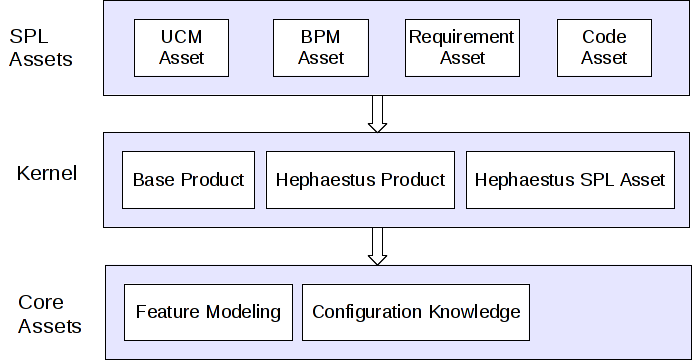
\includegraphics[scale=0.5]{imagens/architecture-hpl.png}
\end{center}
\caption{Hephaestus-PL's architecture}
\label{fig:architecture-hpl}
\end{figure*}

%%%%%%%%%%%%%%%%%%%%%%%%%%%%%%%%%%%%%%%%%%%%%%%%%%

In order to achieve the key requirements of configurability and flexibility in product derivation tools such as \hp{}, we proposed the development of these tools as product lines themselves, in this case~\hpl{} as a product live over existing \hp{} variants, and a transformational approach to variability management within these product lines. To realize the domain model identified in Section~\ref{sec:domainAnalysis} and thus manage the underlying variability, the design of \hpl{} comprises the architecture depicted in Figure~\ref{fig:architecture-hpl}. Key in this architecture is the \textit{Kernel} representing the minimum structure necessary for generation of product \hpl{} instances besides generating itself in a bootstrapping process. Within the kernel, \emph{Base Product} represents the commonality among all \hpl{}'s instances and it has variability points which are resolved by transformations defined in \emph{\hp{} SPL Asset}, in a derivation process driven by \emph{\hp{} Product}.

Besides the \textit{Kernel}, \hpl's architecture also presents the \textit{Core Assets} and \textit{SPL Assets} which contribute to the kernel in the generation of \hpl{} instances. \textit{Core Assets} contains the definition of the representation of the Feature Model and Configuration Knowledge which are key elements of a \hpl{} instance in the product derivation process. \textit{SPL Assets} represents the definition of each asset and corresponding transformations allowing the generation of \hpl{} instances that support variability management and the derivation of products in the domain of these assets. In Subsection~\ref{architectural-elements-hpl}, we present details on the elements depicted in the Figure~\ref{fig:architecture-hpl}.

We adopt a transformational approach~\cite{deltaSchaefer} to variability management because of the expressiveness needed to address the heterogeneity of the variability patterns observed in Section~\ref{domain-analysis-hpl} without compromising modularity and comprehensibility, and thus flexibility, which are issues in annotative approaches~\cite{kastner:2008}. Although these patterns involve scattering and tangling, a compositional approach (e.g., AOP) does not meet the expressiveness requirement given the heterogeneity in granularity. With this transformational approach, 1) configurability is addressed by enabling \hpl{} with an automatic support to generate product instances with different combinations of assets; 2) flexibility is guaranteed by \hpl{}'s architectural design allowing support to variability management of different assets, independence between the assets and mostly no impact on kernel when inserting new assets in \hpl.

%As result of the domain analysis were defined the base product, the transformations to the variability management, the feature modeling and the configuration knowledge of \hpl{}.

%Figure~\ref{fig:apis-hpl-asset} shows that each \hpl's transformation (high level API) was implemented with a set of transformations in Haskell code (low level API) implemented by operations of metaprogramming that solve the variation points in the base product. Both high and low level API were defined from the domain analysis and the variability analysis in \hpl{}.
%From a selected product configuration, the kernel of \hpl{} runs the refinement of the base product using the transformations of \hpl{} (high level API) contained in CK corresponding to the selected features, which in turn, invoke the Haskell code transformations (low level API) implemented by operations of metaprogramming that solve the variability in the base product for the selected feature. Both high- and low-level APIs were defined from the domain analysis and the variability analysis in \hpl{} and the APIs represent the suport to the \hpl{} kernel.

%%%%%%%%%%%%%%%%%%%%%%%%%%%%%%%%%%%%%%%%%%%%%%%%%%

\subsection{\hpl's Product Derivation Process} \label{product-derivation-hpl}

To illustrate a key scenario of \hpl's product derivation process, suppose a specific feature configuration (FC) contains four features: use case model (\emph{UseCase}), business process model (\emph{BusinessProcess}), use case in xml format (\emph{UcmToXML}), and business process in xml format (\emph{BpmToXML}), as shown in the Figure~\ref{fig:fc-ucm-bpm}.

%%%%%%%%%%%%%%%%%%%%%%%%%%%%%%%%%%%%%%%%%%%%%%%%%%

\begin{figure*}[bth]
\begin{center}
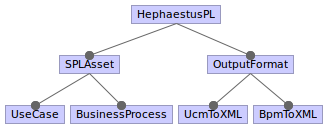
\includegraphics[scale=0.8]{imagens/fc-ucm-bpm.png}
\end{center}
\caption{\hpl's feature configuration to generate a \hpl's instance}
\label{fig:fc-ucm-bpm}
\end{figure*}

%%%%%%%%%%%%%%%%%%%%%%%%%%%%%%%%%%%%%%%%%%%%%%%%%%

\hpl's product derivation process is based on \hpl's Configuration Knowledge (CK), an excerpt of which is shown in Table~\ref{tab:ck-hpl}.  This CK relates feature expressions to transformations that solve \hpl{}'s variability.  As shown in the \textit{transformations} column of Table~\ref{tab:ck-hpl}, we defined \hpl's transformations which are detailed in Subsection~\ref{hephaestus-spl-asset}, and when applied they progressively bind variability in the base product (cf. Figure~\ref{fig:derivationHPL}) as \hpl's instance is generated.


%\begin{figure*}[bth]
%\begin{center}
%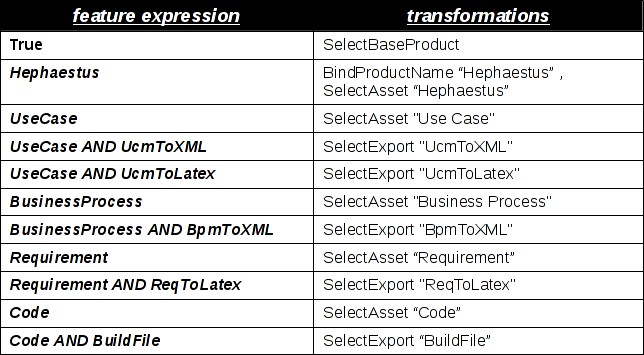
\includegraphics[scale=0.6]{imagens/ck-hpl.png}
%\end{center}
%\caption{\hpl's Configuration Knowledge}
%\label{fig:ck-hpl}
%\end{figure*}

%%%%%%%%%%%%%%%%%%%%%%%%%%%%%%%%%%%%%%%%%%%%%%%%%%

\begin{table}[h]
\begin{center}
\begin{tabular}{||l||l||}
  \hline
  \textbf{Feature Expressions} & \textbf{Transformations}   \\  \hline
  True & SelectBaseProduct \\  \hline
%  Hephaestus & BindProductName "Hephaestus" \\
%             &  SelectAsset "Hephaestus"   \\
%             &  RemoveProductMainFunction \\ \hline
%  NOT Hephaestus & SelectCKParser \\ \hline
  UseCase & SelectAsset "Use Case" \\ \hline
  UseCase AND UcmToXML & SelectExport "UcmToXML"  \\ \hline
  UseCase AND UcmToLatex & SelectExport "UcmToLatex" \\ \hline
  BusinessProcess & SelectAsset "Business Process" \\ \hline
  BusinessProcess AND BpmToXML & SelectExport "BpmToXML" \\ \hline
  Requirement & SelectAsset "Requirement" \\ \hline
  Requirement AND ReqToLatex & SelectExport "ReqToLatex" \\ \hline
  Code & SelectAsset "Code" \\ \hline
  Code AND BuildFile & SelectExport "BuildFile" \\ \hline
\end{tabular}
\caption{Excerpt \hpl's Configuration Knowledge}
\label{tab:ck-hpl}
\end{center}
\end{table}

%%%%%%%%%%%%%%%%%%%%%%%%%%%%%%%%%%%%%%%%%%%%%%%%%%

Figure~\ref{fig:derivationHPL} abstractly depicts the steps taken in \hpl's product derivation process considering the feature configuration shown in  Figure~\ref{fig:fc-ucm-bpm}. \hpl{}'s CK (Table~\ref{tab:ck-hpl}) guides this transformational process in five steps towards the generation of a \hpl{} instance from the base product. \hpl{}'s CK is evaluated from first to last row, triggering execution of only those transformations whose corresponding feature expression evaluates to true according to the given configuration.

%%%%%%%%%%%%%%%%%%%%%%%%%%%%%%%%%%%%%%%%%%%%%%%%%%

\begin{figure*}[bth]
\begin{center}
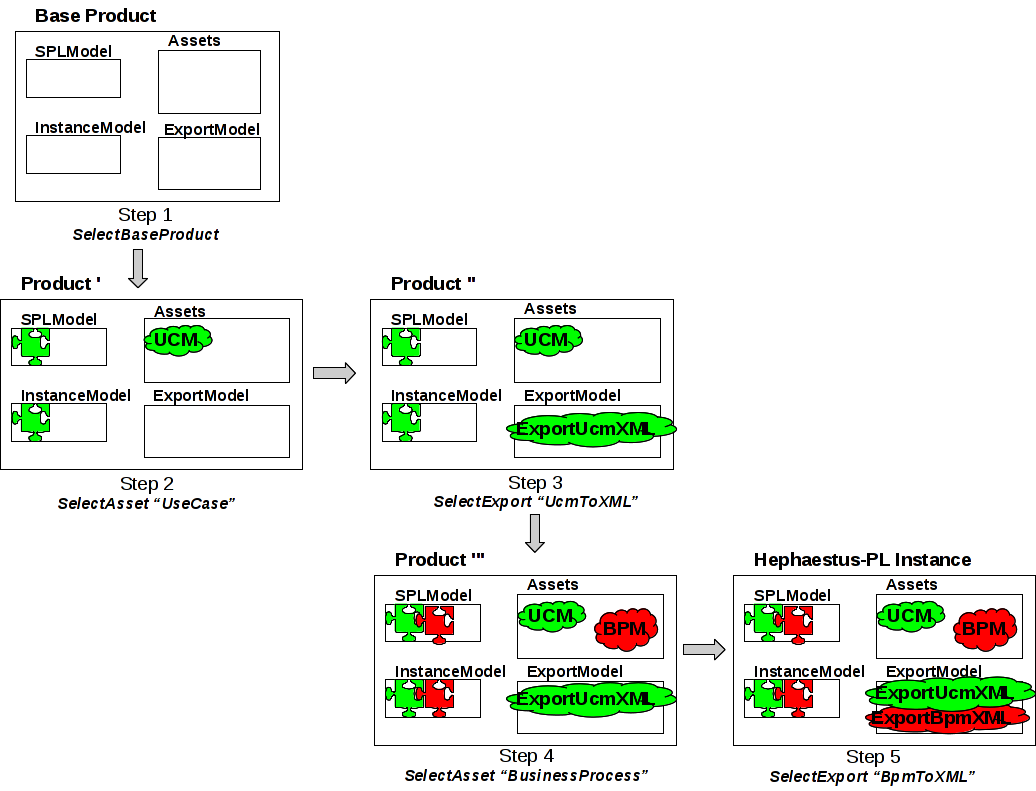
\includegraphics[width=\textwidth]{imagens/derivation.png}
\end{center}
\caption{Derivation of an Hephaestus-PL instance supporting the UCM, BPM, UcmToXML and BpmToXML features.}
\label{fig:derivationHPL}
\end{figure*}

%%%%%%%%%%%%%%%%%%%%%%%%%%%%%%%%%%%%%%%%%%%%%%%%%%

Accordingly, \hpl's product derivation process begins with the execution of the \texttt{SelectBaseProduct} transformation associated with
the feature expression \texttt{True} in the first line of \hpl's CK (Table ~\ref{tab:ck-hpl}). Indeed,
this transformation is always executed at the beginning of the generation of a new \hpl{} instance and represents the selection of the base product that contains the commonality of any \hpl{} instance.

%
%Next, since the configuration does not contain feature \emph{Hephaestus} and thus the feature expression in the second line of the evaluated to false according to the configuration, the transformations on such line are not executed. On the other hand, as the feature expression in the third line () evaluates to true according to the configuration, the corresponding transformation is executed: SelectCKParser.

Next, in the second line of \hpl's CK, the \texttt{UseCase} feature expression evaluates to true according to the FC shown in Figure~\ref{fig:fc-ucm-bpm} and thus the \texttt{SelectAsset "Use Case"} transformation is executed: it performs a set of transformations in the base product, binding variation points of the base product by adding components of the \textit{UCM Asset}(Step 2 in Figure~\ref{fig:derivationHPL}).  More specifically, the transformation introduces the UCM asset data type as field into the \texttt{SPLModel} and \texttt{InstanceModel} data types and imports the modules that define the UCM data types and corresponding transformations.  Following in the Step 3, feature expression \texttt{UseCase AND UcmToXML} evaluates to true in the third line of \hpl's CK and then the \texttt{SelectExport "UcmToXML"} transformation is executed. This transformation extends the product under derivation, adding components of the \textit{UCM Asset} to support the exportation of use cases in the XML format, i.e., introduces the \texttt{ExportUcmXML} constructor corresponding to \textit{UcmToXML} feature into \texttt{ExportModel} data type and adds the module that implements use case's xml output format into Product'.

Steps 4 and 5 then execute similar transformations in the product under derivation to those performed by Steps 2 and 3 described previously.  Therefore, the \texttt{BusinessProcess} and \texttt{BusinessProcess AND BpmToXML} feature expressions evaluate to true according to the configuration. As a result, the corresponding transformations in the CK bind some more of the remaining variation points of the product under derivation by adding components of the \textit{BPM Asset} into this product to support the variability management and export capability of business process model in the generated \hpl{} instance.

We note that both \textit{UCM Asset} and \textit{BPM Asset} are architectural elements belonging to \textit{SPL Assets}, as represented in Figure~\ref{fig:architecture-hpl}.

%First, in Step 1, the process begins with the selection of the Base Product that contains the commonality of a \hpl{} instance. This base instance of Hephaestus-PL is obtained from the \texttt{SelectBaseProduct} transformation associated with the feature expression \texttt{True} in the first line of the \hpl{} CK (see Figure~\ref{fig:hpl-ck}), e.g., it will always be executed at the beginning of the generation of a new instance of Hephaestus-PL and thus is a key core asset.

%The Base Product will be extended to compose an instance of Hephaestus with the assets of interest.
%These statements and functions that will be extended from the selected assets in Hephaestus-PL we call the open data types and open functions.
%The underlying metaprogramming operation in SelectBaseProduct is setModuleName, which  defines the name of empty module of the new instance of Hephaestus.

%Next, Step 2 represents the result generated by selecting the \emph{Use Case} feature and the incurred application of the \texttt{SelectAsset "Use Case"} transformation that performs a set of transformations in the base product, adding artifacts (elements in green color) of the selected UCM asset in the base product. More specifically, we apply the metaprogramming operations to introduce the UCM asset data type as fields into the \texttt{SPLModel} and \texttt{InstanceModel} data types, to import the modules that implements the use case model data types, the use case model transformations and the parser of the UCM asset into the base product, to add the empty UCM into the \emph{empty instance} function, to add the transformations of the UCM into configuration knowledge XML parser and to evolve the \emph{main} function.
	
%Then, in Step 3 we have the selection of the \emph{Business Process} feature and, consequently, the execution of the \texttt{SelectAsset "Business Process"} transformation that performs similar changes in the module of Hephaestus being generated when compared to the selection of the \emph{Use Case} feature, the difference now being the BPM asset (elements represented in red).

%In Step 4, we have the selection of the \emph{UcmToXML} feature, which prompts the execution of the \texttt{SelectExport "UcmToXML"} transformation, which the extends the Hephaestus product being constructed to support the exportation of use cases in the XML format, i.e., extends the \texttt{ExportModel} data type, the \texttt{lstExport} list and the \texttt{export} function, besides adding the module that implements the use case xml output format into the base product. The \texttt{SelectExport <assetNameFormat>} transformation associated with the feature expression \emph{assetName AND assetNameFormat} performs transformations in the Hephaestus product being generated also using meta-programming operators (for type and function extension).

%Finally, in Step 5 we have the selection of the \emph{BpmToXML} feature and, consequently, the execution of the \texttt{SelectExport "BpmToXML"} transformation that performs similar changes in the base product of Hephaestus instance being generated when compared to the selection of the \emph{UcmToXML} feature outlined above.

%%%%%%%%%%%%%%%%%%%%%%%%%%%%%%%%%%%%%%%%%%%%%%%%%%

\subsection{\hpl's Architectural Elements} \label{architectural-elements-hpl}

In what follows we detail the main building blocks of \hpl{}'s architecture with emphasis on the kernel and its related elements (Core Assets and SPL Assets).  The kernel consists of three elements: \hp{} Product (Section~\ref{hephaestus-product}), \hp{} SPL Asset (Section~\ref{hephaestus-spl-asset}), and Base Product (Section~\ref{base-product}). Together these elements comprise the minimal structure responsible for generating instances of \hpl{} products. Further, they have a certain degree of coupling and are mostly stable with respect to evolution of \hpl{}. Sections~\ref{spl-assets} and~\ref{core-assets} describe SPL Assets and Core Assets, respectively.

%%%%%%%%%%%%%%%%%%%%%%%%%%%%%%%%%%%%%%%%%%%%%%%%%%

\subsubsection{Hephaestus Product} \label{hephaestus-product}

\hp{} Product is a minimal \hpl{} instance that only supports variability management of \hp{} SPL Asset and corresponds to a Haskell module that could be generated by bootstrapping, i.e., \hp{} Product could be used to generate itself, in which case the \hp{} feature is selected in a configuration of \hpl's FM.

Managing variability of \hp{} SPL Asset means that \hp{} Product is used to derive products according to \hpl{}'s variability space. Indeed, this module declares the \texttt{build} function, which controls \hpl{}'s product derivation process--by progressive refinement of the base product--and provides a simple definition for the \texttt{transform} function (code snippet in the Figure~\ref{fig:code-hp-product}).  In this particular instance, the \texttt{transform} function only deals with the transformations of the \hp{} SPL Asset, which are detailed in Section~\ref{hephaestus-spl-asset}.

%%%%%%%%%%%%%%%%%%%%%%%%%%%%%%%%%%%%%%%%%%%%%%%%%%

\begin{figure}
%\begin{code}
\begin{lstlisting}
build :: FeatureModel
      -> FeatureConfiguration
      -> ConfigurationKnowledge
      -> SPLModel
      -> InstanceModel

build fm fc ck spl = stepRefinement ts spl emptyInstance
  where emptyInstance = mkEmptyInstance fc spl
        ts = tasks ck fc

tasks :: ConfigurationKnowledge -> FeatureConfiguration -> [TransformationModel]
tasks ck fc = concat [transformations c | c <- ck, eval fc (expression c)]

transform :: TransformationModel -> SPLModel -> InstanceModel -> InstanceModel
transform (HephaestusTransformation t) s i = transformHpl t s i
\end{lstlisting}
%\end{code}
\caption{Code snippet of the \hp{} product}
\label{fig:code-hp-product}
%\end{code}
\end{figure}

%%%%%%%%%%%%%%%%%%%%%%%%%%%%%%%%%%%%%%%%%%%%%%%%%%

%
%\subsubsection{Hephaestus-PL's FM and CK}
%
%The instances of the feature model (FM) and configuration knowledge (CK) of \hpl{} are key inputs in the \texttt{build} process of the \hp{} product to derive new products.
%
%%A Haskell module that declares instances for both \hpl{} feature model and configuration knowledge.
%
%This feature model declares the variability space of \hpl{}, as Figure~\ref{fig:hephaestus-fm-03}
%details, while the \hpl{'s} configuration knowledge relates feature
%expressions to transformations that solves \hpl{} variability. For
%instance, Table~\ref{tab:ck-hpl} shows the configurations items of this
%CK, relating the feature expression
%\texttt{Hephaestus} to the transformations \texttt{BindProductName "Hephaestus"}
%and \texttt{SelectAsset "Hephaestus"}; the feature expression \texttt{UseCase} to
%the transformation \texttt{SelectAsset "UseCase"}; and the feature
%expression \texttt{BusinessProcess} to the transformation
%\texttt{SelectAsset "BusinessProcess"}.
%
%
%Whenever we want to bootstrap \hpl, we derive an instance of \hpl{}
%using a product configuration that has the \texttt{\hp{}} feature. This will
%trigger the product derivation of an intance that manages variability
%of the \hp{} asset. Differently, if we use a product configuration
%that has both \texttt{UseCase} and \texttt{BusinessProcess} features,
%the product derivation will generate an
%\hpl{} instance that manages variability related to these assets.

\subsubsection{Base Product} \label{base-product}

The Base Product is a Haskell module serving as a base for deriving \hpl{} instances. It represents the commonality among \hpl's instances and was obtained as output of \hpl{}'s domain analysis (Section~\ref{domain-analysis-hpl}).  When we build an \hpl{} instance, the derivation process first reads this module and then performs \hp{} asset transformations (mainly \texttt{SelectAsset} and \texttt{SelectExport}), refining several definitions of the \texttt{BaseProduct} module. Figure~\ref{fig:code-hpl-base-product} presents a piece of code of the \texttt{BaseProduct} module, whose definitions are explained in the following:

\begin{itemize}

\item declares basic representations for the \texttt{SPLModel} (lines \ref{splmodelBP-i-1}-\ref{splmodelBP-f-1}) and \texttt{InstanceModel} (lines \ref{instancemodelBP-i-1}-\ref{instancemodelBP-f-1}) data types, where the first
%doest not have any data field
has just the \texttt{featureModel} data field
and the \texttt{InstanceModel} data type has just the \texttt{featureConfiguration} data field,

\item declares \texttt{TransformationModel} data type (line \ref{transformmodelBP}) which just supports the \texttt{UndefinedTransformation} constructor,

\item defines one case for the \texttt{transform} function (lines \ref{transformBP-i-1}-\ref{transformBP-f-1}), which just supports the \texttt{UndefinedTransformation} transformation,

\item declares \texttt{ExportModel} data type (line \ref{exportmodelBP}) which just supports the \texttt{UndefinedExport} constructor,

\item defines an empty list (\texttt{lstExport}) (lines \ref{lstExportBP-i-1}-\ref{lstExportBP-f-1}) of export data types (used to export a product in different output formats),

\item defines one case for the \texttt{export} function (lines \ref{exportBP-i-1}-\ref{exportBP-f-1}), which also just supports the \texttt{UndefinedExport} export format,

\item defines a \texttt{mkEmptyInstance} function (lines \ref{mkEmptyBP-i-1}-\ref{mkEmptyBP-f-1}) that returns an \texttt{InstanceModel} having only the \texttt{featureConfiguration} data field,

\item defines a \texttt{xml2Transformation} function (lines \ref{xm2transfBP-i}-\ref{xm2transfBP-f}) which comprises the CK XML parser process performing the recognition of the concrete syntax of asset transformations of the Hephaestus-PL instance, and

\item defines a \texttt{main} function (lines \ref{mainBP-i-1}-\ref{mainBP-f-1}) to run the \hp{} instance.

\end{itemize}

%The \emph{undefined transformation} could be understood as a hot spot required by the metaprogramming library to introduce new cases of transformations.

The \texttt{TransformationModel} and \texttt{ExportModel} data types could be understood as variation points which will be resolved by introducing new values ​​that will replace the \texttt{UndefinedTransformation} and \texttt{UndefinedExport} definitions, respectively, in the refinement of \hpl{} instance.

%The \texttt{UndefinedTransformation} and \texttt{UndefinedExport} types could be understood as variation points required by the metaprogramming library to introduce new cases of definitions when it is removed in the refinement of \hpl{} instance.

\begin{figure}
%\begin{code}
\begin{lstlisting}
module BaseProduct where

data SPLModel = SPLModel { *'\label{splmodelBP-i-1}'*
  featureModel :: FeatureModel
} *'\label{splmodelBP-f-1}'*

data InstanceModel = InstanceModel { *'\label{instancemodelBP-i-1}'*
  featureConfiguration :: FeatureConfiguration
} deriving (Data, Typeable) *'\label{instancemodelBP-f-1}'*

data TransformationModel = UndefinedTransformation *'\label{transformmodelBP}'*

transform :: TransformationModel -> SPLModel -> InstanceModel -> InstanceModel  *'\label{transformBP-i-1}'*
transform UndefinedTransformation _ _ = undefined  *'\label{transformBP-f-1}'*

data ExportModel = UndefinedExport *'\label{exportmodelBP}'*

lstExport::[ExportModel] *'\label{lstExportBP-i-1}'*
lstExport = []   *'\label{lstExportBP-f-1}'*

export :: ExportModel -> FilePath -> InstanceModel -> IO()  *'\label{exportBP-i-1}'*
export UndefinedExport _ _ = undefined   *'\label{exportBP-f-1}'*

mkEmptyInstance :: FeatureConfiguration -> SPLModel -> InstanceModel  *'\label{mkEmptyBP-i-1}'*
mkEmptyInstance fc spl = InstanceModel {
  featureConfiguration = fc
}    *'\label{mkEmptyBP-f-1}'*

xml2Transformation :: String -> [String] -> ParserResult TransformationModel *'\label{xm2transfBP-i}'*
xml2Transformation "Undefined" _ = undefined *'\label{xm2transfBP-f}'*

main :: IO ()   *'\label{mainBP-i-1}'*
main = do
  ...
  let spl = SPLModel { featureModel = fm }
  let product = undefined  *'\label{build-line}'*
  let out = (outputFile (snd t) (snd n))
  sequence_ [export x out product | x <- lstExport]
  ...   *'\label{mainBP-f-1}'*
\end{lstlisting}
\caption{Code snippet of the \hpl's base product}
\label{fig:code-hpl-base-product}
%\end{code}
\end{figure}

%%%%%%%%%%%%%%%%%%%%%%%%%%%%%%%%%%%%%%%%%%%%%%%%%%

Moreover, instances of \hpl{} must provide one definition for the \texttt{transform} function for each supported SPL asset, even though the product derivation process of \hpl{} refines the \texttt{transform} function introducing those new definitions through metaprogramming.

Line \ref{build-line} of the Figure~\ref{fig:code-hpl-base-product} represents a \texttt{undefined} \hpl's instance (\texttt{product} variable) and this line will be replaced in emerging product by the line \texttt{let product = build fm fc cm spl} that executes the \texttt{build} function to generation of a product \hpl{} instance from feature configuration.

%The \texttt{xm2Transformation} definition (lines \ref{xm2-transf-i}-\ref{xm2-transf-f} of the Figure~\ref{fig:code-hpl-base-product}) comprises the CK parser process performing the recognition of the concrete syntax of asset transformations of the Hephaestus-PL instance.

%%%%%%%%%%%%%%%%%%%%%%%%%%%%%%%%%%%%%%%%%%%%%%%%%%

\subsubsection{Hephaestus SPL Asset} \label{hephaestus-spl-asset}

This element declares algebraic data types representing \hp{} SPL asset, which just corresponds to a list of Haskell modules and the set of transformations for managing \hpl{} variability (code snippet in Figure~\ref{fig:code-hp-spl-asset}). In essence, these transformations are responsible for the refinement of the base product during derivation of the \hpl{} instance. In addition, this module also declares the \texttt{transformHpl} function which is responsible for actually performing the corresponding \hpl{} transformations and it has the same signature of \texttt{transform} function declared in the \hp{} product described in Section~\ref{hephaestus-product}.

Considering the configurability and flexibility requirements driving \hpl's design, we employed a layered design as depicted in Figure~\ref{fig:apis-hpl-asset}: we defined in \hp{} SPL Asset two sets of transformations: \hpl{} transformations (or high-level API) and metaprogramming operations (or low-level API). Each \hpl{} transformation is implemented using the services of metaprogramming operations.
%This complies with the layered model where the low-level API provides services to the high-level API as depicted in Figure~\ref{fig:apis-hpl-asset}.
The design of each layer was guided by domain analysis in terms of implementation assets: the high-level API was guided by the outcome of \hpl{}'s domain analysis  (Section~\ref{domain-analysis-hpl}), whereas  the low-level API, by the domain analysis of the high-level API. Further details in Section~\ref{sec:metaprogrammingOperations}.

%%%%%%%%%%%%%%%%%%%%%%%%%%%%%%%%%%%%%%%%%%%%%%%%%%

\begin{center}
\begin{figure}[htb]
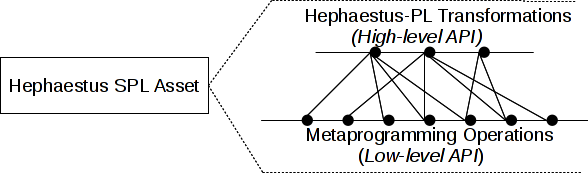
\includegraphics[scale=0.7]{imagens/apis-hpl-asset.png}
\caption{Logical view of the \hpl's APIs}
\label{fig:apis-hpl-asset}
\end{figure}
\end{center}

%In essence, these transformations are built on top of a
%metaprogamming library that evolves a set of minimal \hp{} modules in order to derive
%an \hpl{} instance.

%%%%%%%%%%%%%%%%%%%%%%%%%%%%%%%%%%%%%%%%%%%%%%%%%%

\begin{figure}
%\begin{code}
\begin{lstlisting}
data HephaestusModel = HephaestusModel [HsModule]

data HephaestusTransformation = SelectBaseProduct
                              | SelectAsset String
                              | SelectExport String
                              | BindProductName String
                              | RemoveProductMainFunction
                              | SelectCKParser

transformHpl :: HephaestusTransformation
             -> SPLModel
             -> InstanceModel
             -> InstanceModel
\end{lstlisting}
\caption{Code snippet of the Hephaestus SPL Asset}
\label{fig:code-hp-spl-asset}
%\end{code}
\end{figure}

%%%%%%%%%%%%%%%%%%%%%%%%%%%%%%%%%%%%%%%%%%%%%%%%%%

We defined six \hpl{} transformations, which are represented by the following type constructors:

\begin{itemize}

\item \texttt{SelectBaseProduct} is always the first transformation to be executed in the process of deriving a \hpl{} instance. This transformation selects a \hpl{} base product that represents the commonality of a \hpl{} product. The base product is detailed in section~\ref{base-product}.

\item \texttt{SelectAsset} refines the product being derived with support for the selected asset variability as described by the feature configuration, i.e., this transformation extends the \texttt{SPLModel}, \texttt{InstanceModel} and \texttt{TransformationModel} data types and the \texttt{transform}, \texttt{xml2Transformation}, and \texttt{mkEmptyInstance} (empty instance definition to \texttt{build} function) functions to manipulate such asset. Furthermore, it incorporates the modules defining algebraic data types, the transformations, and the parser of the selected asset in the product being derived.  It also performs extensions into \texttt{main} function introducing the asset parser instruction and extending the instance of \texttt{SPLModel} data type with the asset selected to the \texttt{build} process.

\item \texttt{SelectExport} refines the product being derived with support for the selected output format by extending the \texttt{ExportModel} data type, the \texttt{lstExport} list definition and the \texttt{export} function. Furthermore, it incorporates the module implementing the selected output format function into the product being derived. We define different transformations as \texttt{SelectAsset} and \texttt{SelectExport} to represent the refinement on the base product because the set of metaprogramming operations associated with each of these \hpl{} transformations is different and independent.

\item \texttt{BindProductName} sets \hpl{}'s instance module name.
%Is only used when the \hp{} feature is in a configuration of \hpl's FM.

\item \texttt{RemoveProductMainFunction} is only used when the \hp{} feature is in a configuration of \hpl's FM. This transformation removes the definition of the \texttt{main} function from the product being derived because the \hp{} feature uses the \texttt{buildHpl} function located in another module instead.

\item \texttt{SelectCKParser} refines the product being derived with the CK parser by introducing sentences into the \texttt{main} function to execute the parsing of \hpl's instance CK and changing the \texttt{product} declaration from \texttt{undefined} to \texttt{build fm fc cm spl}, which refers to the CK defined by the \texttt{SelectCKParser} transformation. Furthermore, it incorporates the module defining the CK XML parser into the emerging product. This transformation is only applied to the \texttt{NOT \hp{}} feature expression. When \texttt{\hp{}} feature is selected, such transformation is not applied because the instance corresponding to this feature is the Hephaestus product and the transformations for managing variability within it are precisely the transformations described in this bullet list, which are referred to from the Hephaestus product and thus do not need to be parsed.
    %the CK definition to \hp{} feature is already located into MetaData.hs module and it does not use parser.
\end{itemize}

%%%%%%%%%%%%%%%%%%%%%%%%%%%%%%%%%%%%%%%%%%%%%%%%%%

\subsubsection{SPL Assets} \label{spl-assets}

Define the artifacts for each SPL asset, i.e., the algebraic data types representing a SPL asset, the set of transformations for solving asset's variability and the parser function to convert the external format into algebraic data types defined to \hpl.

In addition, this module also needs to define a data type and a function that comprising all asset's transformations to be used in \texttt{transform} function in the refinement of the base product when the asset is selected, for example, \texttt{UseCaseTransformation} data type and \texttt{transformUcm} function to the \texttt{Use Case} asset. The \texttt{transformUcm} function must have the same signature of \texttt{transform} function declared in the base product described in Section~\ref{base-product}.

% we employed a bootstrapping  approach, such that a kernel \hpl{}
% bootstraps itself and also generates all other kinds of \hp,
% each addressing variability in a different combination of artifacts,
% as seen in Figure~\ref{fig:bootstrap}.
% The bootstrapping approach was applied, since it is a well-known
% design approach to investigate
% the expressivity of tools and languages, allowing us to reuse key
% components in the different variants of \hp{} as well as to increase its configurability and flexibility.

% Indeed, the kernel is a domain asset, manipulates other domain assets
% modeling the tool space (artifacts, transformations
% related to these artifacts, and the tool itself) and builds the
% products, i.e., \hp{}
% variants, corresponding to a given configuration specifying the
% artifacts the current product deals with.
% Since Hephaestus-PL was bootstrapped from such independent versions
% of Hephaestus,  Hephaestus-PL's CK, as well as Hephaestus's CK, represents a mapping of feature expressions to  transformations.

% In particular, a given \hpl{} configuration triggers execution of
% high-level transformations according to \hpl's CK (e.g.,
% \texttt{SelectAsset} and \texttt{SelectExport}).
% These transformations extend the domain \emph{Empty Product}, i.e., a
% module containing reusable declarations and empty or partially defined
% functions, to a product instance.
% Such transformations rely on meta programming support provided by a
% module whose interface specifies
% operations for opening up data types and functions, selecting types
% describing artifacts and the tool itself (details are described in Section~\ref{sec:implementation}).


% \begin{figure*}[bth]
% \begin{center}
% 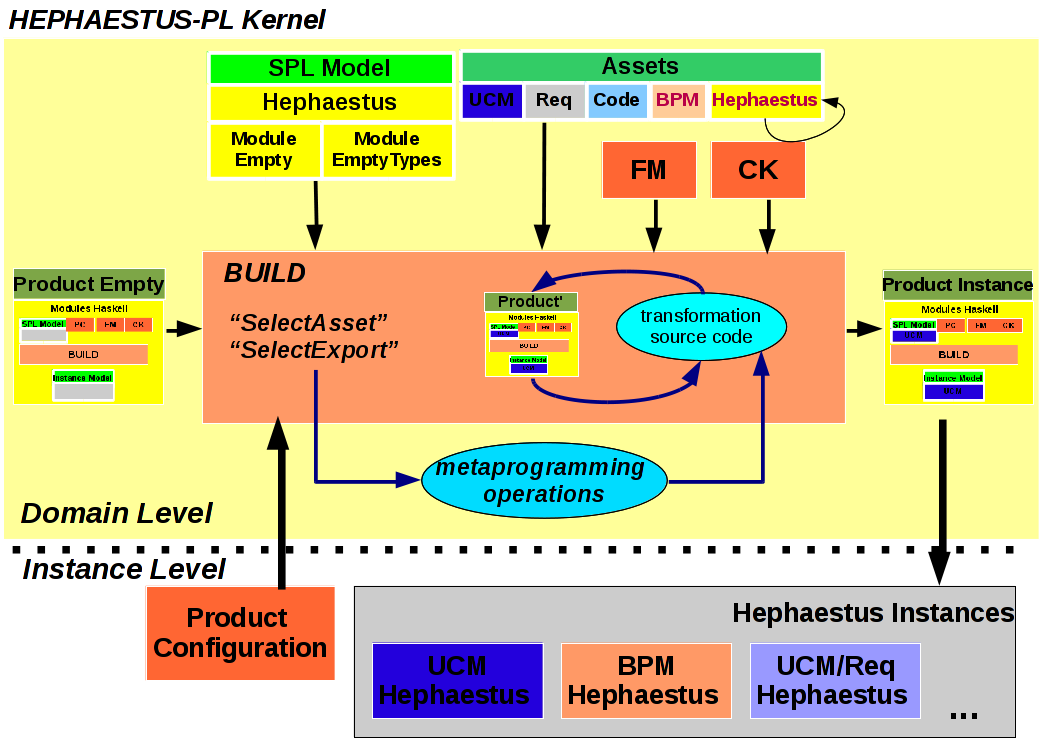
\includegraphics[scale=0.5]{imagens/architecture.png}
% \end{center}
% \caption{Bootstrapping in \hpl.}
% \label{fig:bootstrap}
% \end{figure*}

%%%%%%%%%%%%%%%%%%%%%%%%%%%%%%%%%%%%%%%%%%%%%%%%%%

\subsubsection{Core Assets} \label{core-assets}

These are Haskell modules that declare algebraic data types for representing feature modeling (FM) and configuration knowledge (CK) assets, as well as functions for type checking and other types of verification for these assets. Indeed, these modules were completly reused from the previous versions of \hp. For this reason, \hpl{} instances share these assets as they are declared in the core assets of \hpl--- no transformations on these assets are necessary.

The instances of the \hpl{}'s FM and CK are key inputs in the \texttt{build} process of \textit{\hp{} Product} to derive new \hpl{} instances.

%A Haskell module that declares instances for both \hpl{} feature model and configuration knowledge. 

The \hpl{}'s FM declares the variability space of \hpl{}, as shown in Figure~\ref{fig:hephaestus-fm-03}.  The whole \hpl{'s} CK is represented by Table~\ref{tab:ck-hpl} adding the lines related to \texttt{\hp{}} feature as shown in the Table~\ref{tab:ck-hpl-2}.

%%%%%%%%%%%%%%%%%%%%%%%%%%%%%%%%%%%%%%%%%%%%%%%%%%

\begin{table}[h]
\begin{center}
\begin{tabular}{||l||l||}
  \hline
  \textbf{Feature Expressions} & \textbf{Transformations}   \\  \hline
  Hephaestus & BindProductName "Hephaestus" \\
             &  SelectAsset "Hephaestus"   \\
             &  RemoveProductMainFunction \\ \hline
  NOT Hephaestus & SelectCKParser \\ \hline
\end{tabular}
\caption{Lines of \hpl's CK related to \texttt{\hp{}} feature}
\label{tab:ck-hpl-2}
\end{center}
\end{table}

%%%%%%%%%%%%%%%%%%%%%%%%%%%%%%%%%%%%%%%%%%%%%%%%%%

Whenever we want to bootstrap \hpl, we derive an instance of \hpl{} using a feature configuration that has only the \texttt{\hp{}} feature. This will trigger the product derivation of an instance that manages variability of the \hp{} asset. Differently, if we use a feature configuration that has both features \texttt{UseCase} and \texttt{BusinessProcess}, the product derivation will generate an \hpl{} instance that manages variability related to these assets.

%%%%%%%%%%%%%%%%%%%%%%%%%%%%%%%%%%%%%%%%%%%%%%%%%%
